\documentclass{article}
    % General document formatting
    \usepackage[margin=0.7in]{geometry}
    \usepackage[parfill]{parskip}
    \usepackage[utf8]{inputenc}
    \usepackage{amsmath}
    \usepackage{amssymb}
    \usepackage{tikz}
    \usepackage{fancyhdr}
    \usepackage{listings}
    \usepackage{multicol}

\pagestyle{fancy}
\fancyhf{}
\rhead{Edgar Jacob Rivera Rios - A01184125}

\begin{document}
\begin{titlepage}

    \newcommand{\HRule}{\rule{\linewidth}{0.5mm}} % Defines a new command for the horizontal lines, change thickness here

    \center % Center everything on the page

    %----------------------------------------------------------------------------------------
    %	HEADING SECTIONS
    %----------------------------------------------------------------------------------------

    \textsc{\LARGE Tecnológico de Monterrey}\\[1.5cm] % Name of your university/college
    \textsc{\Large Computational intelligence}\\[0.5cm] % Major heading such as course name
    %\textsc{\large Minor Heading}\\[0.5cm] % Minor heading such as course title

    %----------------------------------------------------------------------------------------
    %	TITLE SECTION
    %----------------------------------------------------------------------------------------

    \HRule \\[0.4cm]
    { \huge \bfseries Activity Extra Point}\\[0.4cm] % Title of your document
    \HRule \\[1.5cm]

    %----------------------------------------------------------------------------------------
    %	AUTHOR SECTION
    %----------------------------------------------------------------------------------------

    \begin{minipage}{0.4\textwidth}
    \begin{flushleft} \large
    \emph{Student:}\\
    Jacob \textsc{Rivera} % Your name
    \end{flushleft}
    \end{minipage}
    ~
    \begin{minipage}{0.4\textwidth}
    \begin{flushright} \large
    \emph{Professor:} \\
    Dr. José Carlos \textsc{Bayliss} % Supervisor's Name
    \end{flushright}
    \end{minipage}\\[2cm]

    % If you don't want a supervisor, uncomment the two lines below and remove the section above
    %\Large \emph{Author:}\\
    %John \textsc{Smith}\\[3cm] % Your name

    %----------------------------------------------------------------------------------------
    %	DATE SECTION
    %----------------------------------------------------------------------------------------

    {\large \today}\\[2cm] % Date, change the \today to a set date if you want to be precise

    %----------------------------------------------------------------------------------------
    %	LOGO SECTION
    %----------------------------------------------------------------------------------------

    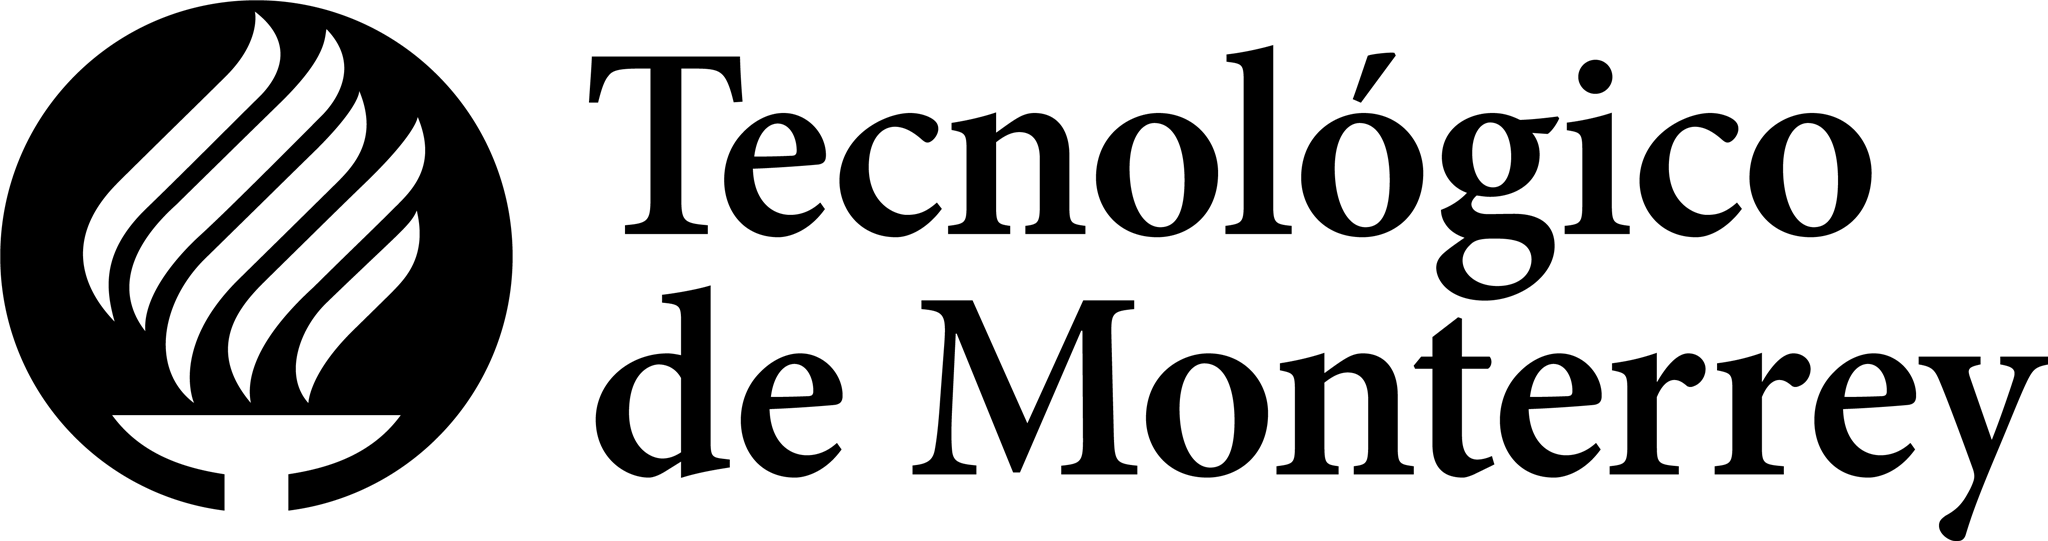
\includegraphics[width=0.4\textwidth,height=\textheight,keepaspectratio]{logo-tec-negro.png} % Include a department/university logo - this will require the graphicx package

    %----------------------------------------------------------------------------------------

    \vfill % Fill the rest of the page with whitespace

\end{titlepage}
\begin{enumerate}
    \item \section*{The eight queens puzzle}
    \begin{itemize}
        \item Propose one suitable chromosome representation and briefly justify your answer.  By using the chromo-some representation you propose, indicate how the chessboard depicted in Fig. 1 would be representedin the genetic algorithm.

        A simple, but useful represantion would be one of a list of integers from 1 to 8, without allowing repetition. In this form, the problem would be even easier to solve as multiple invalid states would be trimmed from the start. And well, the representation of the board shown would be [5,3,1,7,2,8,6,4]

        \item Propose one suitable selection strategy and briefly justify your answer.
        A tournament selection with an m of 4 would probably select very good representations fast as there is not that many options for the list

        \item Propose one suitable crossover operator and briefly justify your answer.

        Using a number between 2 and 6, using it as an index for the first parent, in which numbers to the left of the index would change positions with the equivalents in the second parent. AS

        \item Propose one suitable mutation operator and briefly justify your answer.

        A mutation operator feasible for this representation would change the positions of a pair of items at a selected index. This assures us that it is only a small change but that it gives a noticeable different individual.


    \end{itemize}
    \item \section*{Schemata analysis}
        \begin{table}[h]
            \centering
            \begin{tabular}{l|l|l}
                & Population & $f$ \\
                \hline
                $A_1$ & 10011001  & 4 \\
                $A_2$ & 01101010  & 4 \\
                $A_3$ & 01010111  & 5 \\
                $A_4$ & 01000010  & 2
            \end{tabular}
        \end{table}
        Avg = 3.25
        \begin{table}[h]
            \centering
            \begin{tabular}{l|l|l|l|l|l}
                & Schema & Contained in &count & fitness & f(h) \\
                \hline
                H1& *******1 & $A_1, A_3$ & 2 & 4, 5 & 4.5\\
                H2& *1*****0 & $A_3, A_4$ & 2 & 4, 2 & 3\\
                H3& 0*0****0 & $A_4$ & 1 & 2 & 2\\
                H4& 0******* & $A_2, A_3, A_4$ &3 & 4,5,2 & 3.666\\
            \end{tabular}
        \end{table}

        \subsubsection*{Reproduction}
        \begin{align*}
            m(H_1,t) \frac{f(H_1)}{f}&= 2 *\frac{4.5}{3.75} = 2.4\\
            m(H_2,t) \frac{f(H_2)}{f}&= 2 *\frac{3}{3.75} = 1.6\\
            m(H_3,t) \frac{f(H_3)}{f}&= 1 *\frac{2}{3.75} = 0.53\\
            m(H_4,t) \frac{f(H_4)}{f}&= 3 *\frac{43.6}{3.75} = 2.92\\
        \end{align*}

        \subsubsection*{Crossover}
        Template $\rightarrow$ 01101100
        \begin{multicols}{2}
            $H_1$ = *******1
            \begin{align*}
                Ps &= 1 - (Pc * Pd)\\
                &= 1- 0.8 * 0 = 1
            \end{align*}
            $H2$ = *1*****0
            \begin{align*}
                Ps &= 1 - (Pc * Pd)\\
                &= 1- 0.8 * 1 = 0.2
            \end{align*}
            $H3$ = 0*0****0
            \begin{align*}
                Ps &= 1 - (Pc * Pd)\\
                &= 1- 0.8 * 1 = 0.2
            \end{align*}
            $H4$ = 0*******
            \begin{align*}
                Ps &= 1 - (Pc * Pd)\\
                &= 1- 0.8 * 0 = 1
            \end{align*}
        \end{multicols}

        \subsubsection*{Mutation}
        $Pm = 0.001$
        \begin{multicols}{2}
            $H_1$ = *******1\\
            $O(H_1) = 1$
            \begin{equation*}
                (1-0.001)^1 = 0.999
            \end{equation*}
            $H_2$ = *1*****0\\
            $O(H_2) = 2$
            \begin{equation*}
                (1-0.001)^2 = 0.998
            \end{equation*}
            $H_3$ = 0*0****0\\
            $O(H_3) = 3$
            \begin{equation*}
                (1-0.001)^3 = 0.997
            \end{equation*}
            $H_4$ = 0*******\\
            $O(H_4) = 1$
            \begin{equation*}
                (1-0.001)^2 = 0.999
            \end{equation*}
        \end{multicols}
        \subsection*{Expected number of chromosomes}
        \begin{align*}
            m(H_1,t +1) &= 2.4 * 1 * 0.999 = 2.3975999999999997\\
            m(H_2,t +1) &= 1.6 * 0.2 * 0.998 = 0.3193600000000001\\
            m(H_3,t +1) &= 0.53 * 0.2 * 0.997 = 0.10568200000000001\\
            m(H_4,t +1) &= 2.92 * 1 * 0.999 = 2.91708\\
        \end{align*}
    \item \section*{Steady-state genetic algorithm}

    \item \section*{Analyze the cases}
    \begin{itemize}
        \item Case 1 $\rightarrow$ We should reduce the mutation rate
        \item Case 2 $\rightarrow$ We should increase the population size
        \item Case 3 $\rightarrow$ This is the expected behaviour
    \end{itemize}

\end{enumerate}
\end{document}